\documentclass{article}

% Packages for code listing and syntax highlighting
\usepackage{listings}
\usepackage{xcolor}
\usepackage[margin=3cm]{geometry} % Adjust the margin value as desired
\usepackage{setspace}
\usepackage{tikz}

\onehalfspacing

% Define the color theme
\definecolor{codebackground}{RGB}{242, 242, 242}
\definecolor{codekeyword}{RGB}{0, 0, 255}
\definecolor{codecomment}{RGB}{63, 127, 95}
\definecolor{codestring}{RGB}{163, 21, 21}

% Code listing style for all languages
\lstdefinestyle{mystyle}{
    backgroundcolor=\color{codebackground},
    basicstyle=\footnotesize\ttfamily,
    keywordstyle=\color{codekeyword}\bfseries,
    commentstyle=\color{codecomment}\itshape,
    stringstyle=\color{codestring},
    numbers=left,
    numberstyle=\tiny\color{codecomment},
    stepnumber=1,
    numbersep=8pt,
    showstringspaces=false,
    breaklines=true,
    frame=single,
    frameround=none,
    framesep=5pt,
    rulecolor=\color{codebackground},
    tabsize=4,
    captionpos=b,
    xleftmargin=15pt,
    xrightmargin=15pt
}

% Set the default style for code listings
\lstset{style=mystyle}

% Additional packages and settings for math typesetting
\usepackage{amsmath}
\usepackage{amssymb}
\usepackage{bm}

% Define your document content
\begin{document}

\title{Set Notation}
\author{Abyan Majid}
\date{\today}
\maketitle

\begin{center}
    A set is a collection of objects that are called "elements" of the set.
\end{center}

\par
\noindent A set is denoted as $ A = \{ a_1, a_2, a_3, a_4 \} $, where $a$ is an element of the set $A$. There can be infintely many elements in a set. You can write "..." to denote that a set goes on forever, like so: $ B = \{ b_1, b_2, b_3, ... \} $.

\section{Number sets}
\begin{itemize}
    \item $ \mathbb{N} $ is the set of \textbf{"natural numbers"}: $ \mathbb{N} = \{0, 1, 2, 3, ...\} $ \\ (All positive integers and zero)
    \item $ \mathbb{Z} $ is the set of \textbf{"integers"}: $ \mathbb{Z} = \{..., -3, -2, -1, 0, 1, 2, 3, ...\} $ \\ (All integers and zero)
    \item $ \mathbb{Q} $ is the set of \textbf{"rational numbers"} (eg. $\frac{1}{2}, -\frac{5}{3}, 0.3$) \\ (All numbers of the form $\frac{n}{m}$ where $n$ and $m$ are integers and $m \neq 0$. In other words, all fraction of two integers where the denominator is not $0$.)
    \item $ \mathbb{R} $ is the set of \textbf{"real numbers"}: (eg. $\pi, e, -\sqrt{5}$) \\ (All rational numbers and all irrational numbers) \\ To review: Irrational numbers, such as $\sqrt{2}$ and $\pi$, are numbers that can't be expressed as $\frac{n}{m}$ where $n$ and $m$ are integers.
    \item $ \mathbb{C} $ is the set of \textbf{"complex numbers"}: (eg. $1+2i, 5i, 3+4i$) \\ (Every number set mentioned above combined, plus all imaginary numbers) \\ To review: Imaginary numbers, such as $3i$ and $-2i$, are numbers of the form $bi$, where $b$ is a real number and $i$ is the imaginary unit defined as $\sqrt{-1}$.
\end{itemize}

\section{Two-sets notation}
\begin{itemize}
    \item "$\in$" should be read as \textbf{"is an element of"}
    \item "$\subseteq$" should be read as \textbf{"is a subset of"}
    \item "$\subset$" should be read as \textbf{"is strictly as subset of"}
    \item "$\supseteq$" should be read as \textbf{"contains"}
    \item "$\notin$" should be read as \textbf{"is not an element of"}
    \item "$\not\subseteq$" should be read as \textbf{"is not a subset of"}
    \item "$\cup$" denote the \textbf{union} of two sets, and it is the set of elements of either one or both of the sets. \\ Example: $\{1, 2, 3\}\cup\{3, 4, 5\} = \{1, 2, 3, 4, 5\}$
    \item "$\cap$" denote the \textbf{intersection} of two sets, and it is the set of elements present in both sets. \\ Example: $\{1, 2, 3\}\cap \{2, 3, 4\} = \{2, 3\}$
    \item "$\setminus$" denote the \textbf{subtraction} of one set from another, and it should be read as \textbf{"minus"} or \textbf{"without"} \\ Example: $\{1, 2, 3\}\setminus \{3, 4, 5\} = \{1, 2\}$
\end{itemize}

\section{Interval notation}

An interval is a set of real numbers that lie between two given values. \\

\begin{center}
    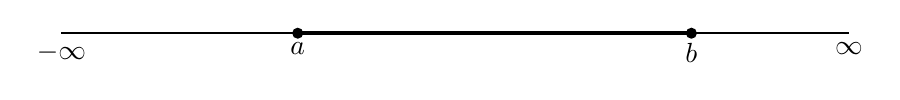
\begin{tikzpicture}
        \draw[-, line width=0.75pt] (-5,0) -- (5,0);
        \coordinate (a) at (-2,0);
        \coordinate (b) at (3,0);
        \draw[-, line width=1.5pt] (a) -- (b);
        \fill (a) circle (2pt) node[below] {$a$};
        \fill (b) circle (2pt) node[below] {$b$};
        \node[below] at (-5, 0) {$-\infty$};
        \node[below] at (5, 0) {$\infty$};
    \end{tikzpicture}
\end{center}

\begin{center}
    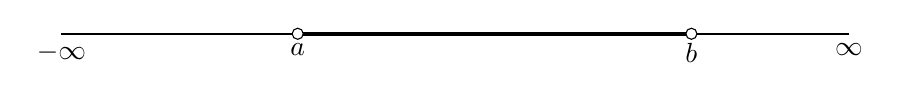
\begin{tikzpicture}
        \draw[-, line width=0.75pt] (-5,0) -- (5,0);
        \coordinate (a) at (-2,0);
        \coordinate (b) at (3,0);
        \draw[-, line width=1.5pt] (a) -- (b);
        \draw[fill=white] (a) circle (2pt) node[below] {$a$};
        \draw[fill=white] (b) circle (2pt) node[below] {$b$};
        \node[below] at (-5, 0) {$-\infty$};
        \node[below] at (5, 0) {$\infty$};
    \end{tikzpicture}
\end{center}

\noindent There's two way in which you can denote an interval:
\begin{enumerate}
    \item First, we can write $\{x\in \mathbb{R} \mid a \leq x \leq b\}$. \\ Here, we're saying $x$ is an element of the set of real numbers $R$ which ranges from and including $a$ and $b$. And, when we do not want to include $a$ and $b$, we write $<$ instead of $\leq$, like so: $\{x\in \mathbb{R} \mid a < x < b\}$
    \item A shorter way to express the interval is by writting $[a, b]$ instead, when $a$ and $b$ are included. When $a$ and $b$ are not included, we can write $(a, b)$.
    
So, in summary: 
\begin{itemize}
    \item "$[$" and "$]$" replaces "$\leq$", denoting that the interval INCLUDES the endpoints.
    \item "$($" and "$)$" replaces "$<$", denoting that the interval does NOT INCLUDE the endpoints.
\end{itemize}

Of course, you can also write $(a, b]$ and $[a, b)$, just as you can write $a < x \leq b$ and $a \leq x < b$
\begin{center}
    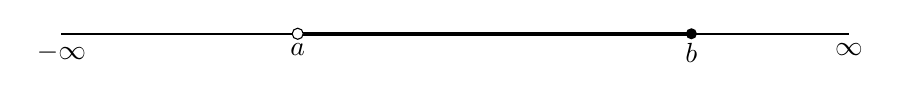
\begin{tikzpicture}
        \draw[-, line width=0.75pt] (-5,0) -- (5,0);
        \coordinate (a) at (-2,0);
        \coordinate (b) at (3,0);
        \draw[-, line width=1.5pt] (a) -- (b);
        \draw[fill=white] (a) circle (2pt) node[below] {$a$};
        \fill (b) circle (2pt) node[below] {$b$};
        \node[below] at (-5, 0) {$-\infty$};
        \node[below] at (5, 0) {$\infty$};
    \end{tikzpicture}
\end{center}

\begin{center}
    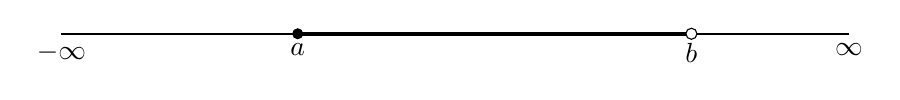
\begin{tikzpicture}
        \draw[-, line width=0.75pt] (-5,0) -- (5,0);
        \coordinate (a) at (-2,0);
        \coordinate (b) at (3,0);
        \draw[-, line width=1.5pt] (a) -- (b);
        \fill (a) circle (2pt) node[below] {$a$};
        \draw[fill=white] (b) circle (2pt) node[below] {$b$};
        \node[below] at (-5, 0) {$-\infty$};
        \node[below] at (5, 0) {$\infty$};
    \end{tikzpicture}
\end{center}

\end{enumerate}


\end{document}